\documentclass[hyperref={bookmarks=false},aspectratio=169]{beamer}
\usepackage{hyperref,ragged2e,amsmath,amssymb,url,bm}
\usepackage{graphicx,booktabs,array}
\usepackage{tikz}
\usetikzlibrary{arrows.meta,positioning,calc,shapes.geometric,decorations.pathreplacing,matrix}
\graphicspath{{crops/}}
\usetheme{Goettingen}
% --- Paleta de la serie Festividades santas: tierra roja, café rojizo, mostaza y papiro ---
\definecolor{tierraroja}{RGB}{122,40,18}
\definecolor{caferojizo}{RGB}{58,18,8}
\definecolor{mostaza}{RGB}{214,160,58}
\definecolor{papiro}{RGB}{243,228,192}
\definecolor{sepia}{RGB}{98,66,44}
\definecolor{oliva}{RGB}{92,98,48}
\setbeamercolor{structure}{fg=tierraroja}
\setbeamertemplate{sidebar canvas right}[vertical shading][top=tierraroja!92!black,bottom=caferojizo]
\setbeamercolor{title in sidebar}{fg=mostaza}
\setbeamercolor{author in sidebar}{fg=papiro}
\setbeamercolor{section in sidebar}{fg=papiro}
\setbeamercolor{section in sidebar shaded}{fg=mostaza!55!papiro!75!tierraroja}
\setbeamercolor{subsection in sidebar}{fg=papiro}
\setbeamercolor{subsection in sidebar shaded}{fg=mostaza!55!papiro!75!tierraroja}
\let\raggedright\justifying
\setlength{\RaggedRightRightskip}{0pt plus 1fil}
\setbeamertemplate{background canvas}{
\includegraphics[width=\paperwidth,height=\paperheight]{papiro.jpg}}
\setbeamercolor{normal text}{fg=caferojizo!90!black}
\setbeamercolor{frametitle}{fg=tierraroja}
\setbeamerfont{frametitle}{series=\bfseries}
\setbeamertemplate{section in toc shaded}{\leavevmode{\color{sepia!85!black}\inserttocsection}\par}
\setbeamercolor{title}{fg=tierraroja}
\setbeamercolor{subtitle}{fg=sepia}
\setbeamercolor{item projected}{bg=tierraroja,fg=papiro}
\setbeamertemplate{itemize item}{\small\textcolor{mostaza!80!tierraroja}{$\blacktriangleright$}}
\setbeamertemplate{navigation symbols}{}
% --- Español + hebreo + griego (XeLaTeX) con fuentes empaquetadas en fonts/ ---
\usepackage[bidi=default]{babel}
\babelprovide[import,main]{spanish}
\babelprovide[import]{hebrew}
\babelprovide[import]{ancientgreek}
\babelfont[hebrew]{sf}[Path=fonts/, BoldFont=NotoHebrewSans-700.ttf]{NotoHebrewSans-400.ttf}
\babelfont[hebrew]{rm}[Path=fonts/, BoldFont=NotoHebrewSans-700.ttf]{NotoHebrewSans-400.ttf}
\babelfont[ancientgreek]{sf}[Path=fonts/]{GFSPorson.otf}
\babelfont[ancientgreek]{rm}[Path=fonts/]{GFSPorson.otf}
\newcommand{\heb}[1]{\mbox{\foreignlanguage{hebrew}{#1}}}
\newcommand{\grc}[1]{\foreignlanguage{ancientgreek}{#1}}
\newcommand{\SENOR}{S{\fontsize{0.78em}{1em}\selectfont EÑOR}}
% --- Citas, imágenes, referencias ---
\usepackage[most]{tcolorbox}
\newtcolorbox{cita}[1][]{enhanced, colback=papiro, opacityback=0.80, colframe=tierraroja!85!mostaza,
  boxrule=0pt, leftrule=2.5pt, arc=0pt, left=6pt, right=6pt, top=4pt, bottom=4pt,
  before skip=4pt, after skip=6pt, fontupper=\small\itshape, #1}
\newcommand{\fuente}[1]{\par\hfill{\upshape\bfseries\footnotesize\textcolor{tierraroja}{#1}}}
\newcommand{\imagen}[3][0.80]{%
  \centering\includegraphics[height=#1\textheight,width=\linewidth,keepaspectratio]{#2}\par\vspace{2pt}
  {\fontsize{5}{6}\selectfont\color{sepia}{\raggedleft\textit{Nota.} #3\par}}}
\makeatletter
\newcommand{\fotolado}[2]{%
  \begin{tikzpicture}[remember picture,overlay]
    \node[anchor=north east,inner sep=0pt] (foto) at ([xshift=-\beamer@sidebarwidth]current page.north east)
      {\includegraphics[height=\paperheight]{#1}};
    \node[anchor=south east,inner sep=2pt,text=papiro,fill=caferojizo,fill opacity=0.55,text opacity=1,
      font=\fontsize{4.5}{5.5}\selectfont,align=right,text width=4.2cm] at ([xshift=-3pt,yshift=3pt]foto.south east)
      {\textit{Nota.} #2};
  \end{tikzpicture}}
\makeatother
\newcommand{\refapa}[1]{\par{\RaggedRight\hangindent=1.2em\hangafter=1\noindent #1\par}\vspace{3pt}}
\usepackage{xurl}\urlstyle{same}
\newcommand{\destacar}[1]{\textbf{\textcolor{tierraroja}{#1}}}
\newcommand{\precision}[1]{{\footnotesize\color{sepia}\textbf{Precisión:} #1}}
\newcolumntype{L}[1]{>{\RaggedRight\arraybackslash}p{#1}}
\tikzset{caja/.style={draw=tierraroja,line width=0.8pt,fill=papiro,fill opacity=0.90,text opacity=1,rounded corners=3pt,inner sep=5pt,font=\scriptsize}}
\title[Shemitá]{\bfseries{Shemitá: el año sabático y el ciclo del siete}}
\subtitle{``El séptimo año la tierra tendrá descanso, reposo para \SENOR'' (Lv 25:4)}
\author{}\institute{}\date{}
\titlegraphic{
\includegraphics[width=0.80\linewidth,height=0.36\textheight,keepaspectratio]{portada.jpg}\\[-1pt]
  {\fontsize{5}{6}\selectfont\color{sepia}\textit{Nota.} Elaboración propia: Lv 25:4a en texto hebreo consonántico (BHS).}}
\begin{document}
\frame{\titlepage}

\begin{frame}\frametitle{Contenidos}\tableofcontents\end{frame}

% ------------------------------------------------------------------
\section{Introducción}

\begin{frame}{Un año que no cabe en el calendario}
\begin{columns}[c,onlytextwidth]
\begin{column}{0.50\textwidth}
\begin{tcolorbox}[colback=papiro,colframe=mostaza,boxrule=1.2pt,arc=3pt]
\centering\itshape La shemitá es el \destacar{sábado de los años}: la tierra descansa, el siervo sale libre, la deuda se suelta.
\end{tcolorbox}
\small\RaggedRight ``¿Qué comeremos el séptimo año?'' (Lv 25:20).\\ ``Cerca está el año séptimo, el de la remisión'' (Dt 15:9).\par\medskip
La Torá pone en palabras las objeciones del campesino y del acreedor, y responde a la primera con una \destacar{promesa} y a la segunda con un \destacar{mandamiento}.
\end{column}
\begin{column}{0.47\textwidth}\small
\begin{itemize}
\item Funda: ``la tierra mía es'' (Lv 25:23).
\item Memorial: ``fuiste siervo en Egipto'' (Dt 15:15).
\item Juicio: la tierra ``gozará sus días de reposo'' en el exilio (Lv 26:34; 2 Cr 36:21).
\item Esperanza: la LXX traduce ``suelta'' y ``libertad'' con \grc{ἄφεσις}, la palabra del \destacar{perdón} (Mt 26:28).
\end{itemize}
\end{column}
\end{columns}
\end{frame}

\begin{frame}{El sábado de Lv 23 se proyecta en los años}
\centering
\resizebox{\linewidth}{!}{%
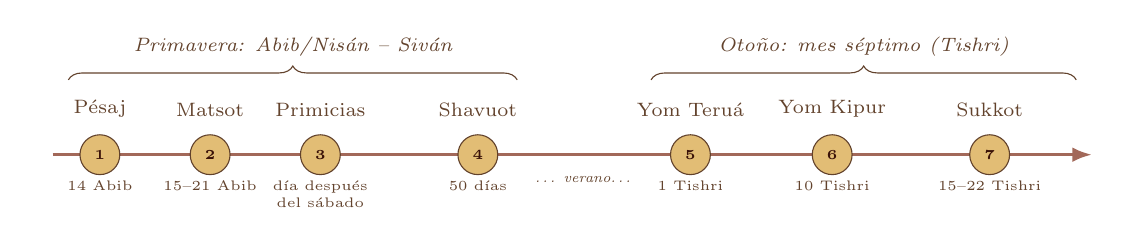
\begin{tikzpicture}[x=1cm,y=1cm,font=\scriptsize]
 \def\fiestaactual{0}
 \draw[line width=1.2pt,tierraroja!70,-{Latex[length=2.5mm]}] (0,0) -- (13.2,0);
 \draw[decorate,decoration={brace,amplitude=5pt},sepia] (0.2,0.95) -- (5.9,0.95) node[midway,above=5pt,font=\scriptsize\itshape]{Primavera: Abib/Nisán -- Siván};
 \draw[decorate,decoration={brace,amplitude=5pt},sepia] (7.6,0.95) -- (13.0,0.95) node[midway,above=5pt,font=\scriptsize\itshape]{Otoño: mes séptimo (Tishri)};
 \foreach \n/\x/\t/\d in {1/0.6/Pésaj/{14 Abib},2/2.0/Matsot/{15--21 Abib},3/3.4/Primicias/{día después del sábado},4/5.4/Shavuot/{50 días},5/8.1/Yom Teruá/{1 Tishri},6/9.9/Yom Kipur/{10 Tishri},7/11.9/Sukkot/{15--22 Tishri}}{
   \ifnum\n=\fiestaactual
     \node[circle,fill=tierraroja,draw=caferojizo,minimum size=5.5mm,text=papiro,font=\scriptsize\bfseries] at (\x,0) {\n};
     \node[above=3pt,font=\scriptsize\bfseries,text=tierraroja] at (\x,0.28) {\t};
   \else
     \node[circle,fill=mostaza!70,draw=sepia,minimum size=4.5mm,text=caferojizo,font=\tiny\bfseries] at (\x,0) {\n};
     \node[above=3pt,text=sepia] at (\x,0.25) {\t};
   \fi
   \node[below=6pt,text width=1.6cm,align=center,font=\tiny,text=sepia] at (\x,0) {\d};}
 \node[font=\tiny\itshape,text=sepia] at (6.75,-0.32) {\ldots\ verano\ldots};
\end{tikzpicture}}\par\medskip
\small\RaggedRight Aquí no se resalta ninguna fiesta, porque la shemitá \destacar{no es un \emph{moed} del año}. Prolonga el primer renglón del reglamento, el sábado (``Seis días se trabajará, mas el séptimo día será de reposo'', Lv 23:3), y lo extiende a los años en el mismo Sinaí (Lv 25:1).\par\smallskip
{\fontsize{5}{6}\selectfont\color{sepia}\textit{Nota.} Esquema estándar de la serie.}
\end{frame}

\begin{frame}{El ciclo de los años}
\begin{columns}[c,onlytextwidth]
\begin{column}{0.52\textwidth}
\centering
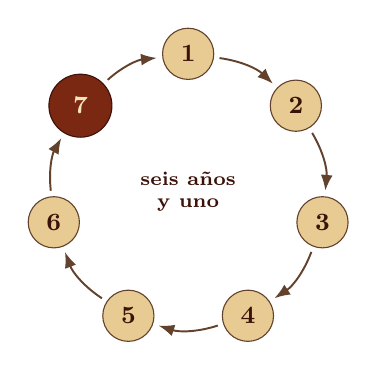
\begin{tikzpicture}[font=\scriptsize]
 \def\R{1.75}
 \foreach \i in {1,...,7}{
   \pgfmathsetmacro{\ang}{90-(\i-1)*360/7}
   \ifnum\i=7
     \node[circle,fill=tierraroja,text=papiro,draw=caferojizo,minimum size=8mm,font=\small\bfseries] (a\i) at (\ang:\R) {7};
   \else
     \node[circle,fill=mostaza!55,draw=sepia,minimum size=6.5mm,text=caferojizo,font=\small\bfseries] (a\i) at (\ang:\R) {\i};
   \fi}
 \foreach \i/\j in {1/2,2/3,3/4,4/5,5/6,6/7,7/1}{\draw[-{Latex[length=2mm]},sepia,line width=0.7pt,shorten >=2pt,shorten <=2pt] (a\i) to[bend left=18] (a\j);}
 \node[align=center,text=caferojizo] at (0,0) {\textbf{seis años}\\\textbf{y uno}};
\end{tikzpicture}
\end{column}
\begin{column}{0.46\textwidth}\small
\begin{itemize}
\item \destacar{Años 1--6}: ``seis años sembrarás tu tierra'' (Lv 25:3).
\item \destacar{Año 7}: \emph{shabat shabatón la'árets} (Lv 25:4); remisión de deudas (Dt 15:1).
\item Fin del año 7, en Sukkot: la Torá leída a todos (Dt 31:10).
\item $7\times7=49$; el año 50, \emph{yovel} (cap. 09).
\end{itemize}
\precision{el siervo de Éx 21:2 cuenta seis años \emph{desde su compra}, no desde este ciclo.}
\end{column}
\end{columns}
\end{frame}

% ------------------------------------------------------------------
\section{Los textos}

\begin{frame}{Texto ancla: Lv 25:1--4}
\fotolado{panel_levitico25.jpg}{Elaboración propia: Lv 25:4 en texto hebreo consonántico (BHS).}
\begin{columns}[c,onlytextwidth]
\begin{column}{0.57\textwidth}
\begin{cita}Cuando hayáis entrado en la tierra que yo os doy, la tierra guardará reposo para \SENOR. Seis años sembrarás tu tierra\ldots{} Pero el séptimo año la tierra tendrá descanso, reposo para \SENOR; no sembrarás tu tierra, ni podarás tu viña.\fuente{(Lv 25:2--4, RVR1960)}\end{cita}
\scriptsize \heb{שַׁבַּת שַׁבָּתוֹן} (\emph{shabat shabatón}): el título del sábado (Lv 23:3) y de Yom Kipur (Lv 16:31). \heb{שַׁבָּת לַיהוָה}: la frase del cuarto mandamiento (Éx 20:10). Aquí la \destacar{tierra es sujeto} del sábado.
\end{column}
\begin{column}{0.41\textwidth}\end{column}
\end{columns}
\end{frame}

\begin{frame}{Éx 23:10--11: la tierra para los pobres}
\begin{center}\heb{וְהַשְּׁבִיעִת תִּשְׁמְטֶנָּה וּנְטַשְׁתָּהּ וְאָכְלוּ אֶבְיֹנֵי עַמֶּךָ}\end{center}
\begin{cita}Seis años sembrarás tu tierra, y recogerás su cosecha; mas el séptimo año la dejarás libre, para que coman los pobres de tu pueblo; y de lo que quedare comerán las bestias del campo; así harás con tu viña y con tu olivar.\fuente{(Éx 23:10--11, RVR1960)}\end{cita}
\small
\begin{itemize}
\item Dos verbos: \heb{תִּשְׁמְטֶנָּה} ``la soltarás'' y \heb{וּנְטַשְׁתָּהּ} ``la abandonarás''.
\item Finalidad declarada: que coman los \heb{אֶבְיֹנֵי עַמֶּךָ}, ``los pobres de tu pueblo'', y los animales.
\item En Lv 25:5--7 lo que nace solo (\emph{sefiaj}) es para \destacar{todos}: dueño, siervo, jornalero, extranjero, ganado.
\end{itemize}
\end{frame}

\begin{frame}{El siervo hebreo sale libre}
\begin{columns}[t,onlytextwidth]
\begin{column}{0.49\textwidth}
\begin{cita}Si comprares siervo hebreo, seis años servirá; mas al séptimo saldrá libre, de balde.\fuente{(Éx 21:2, RVR1960)}\end{cita}
\scriptsize \heb{לַחָפְשִׁי חִנָּם}: ``a la libertad, gratis''. Si elige quedarse, la oreja horadada junto a la puerta: ``será su siervo para siempre'' (21:5--6).
\end{column}
\begin{column}{0.49\textwidth}
\begin{cita}\ldots{}no le enviarás con las manos vacías. Le abastecerás liberalmente de tus ovejas, de tu era y de tu lagar\ldots{} Y te acordarás de que fuiste siervo en la tierra de Egipto\ldots\fuente{(Dt 15:13--15, RVR1960)}\end{cita}
\scriptsize \heb{הַעֲנֵיק תַּעֲנִיק}: ``le cargarás el cuello'' (\emph{anaq}, ``collar''). Deuteronomio añade a la \destacar{hebrea}, llama al siervo \destacar{``tu hermano''} y exige \destacar{provisión}.
\end{column}
\end{columns}
\end{frame}

\begin{frame}{``¿Qué comeremos?'' (Lv 25:20--22)}
\begin{cita}Y si dijereis: ¿Qué comeremos el séptimo año?\ldots{} entonces yo os enviaré mi bendición el sexto año, y ella hará que haya fruto por tres años.\fuente{(Lv 25:20--21, RVR1960)}\end{cita}
\centering
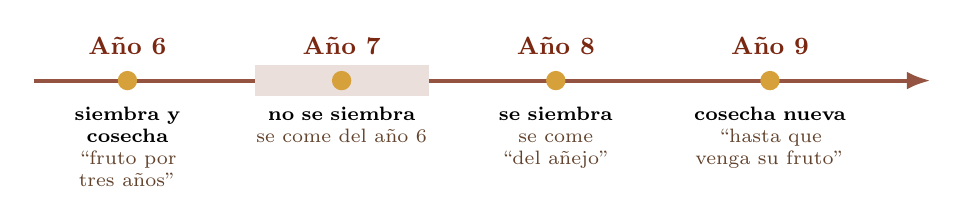
\begin{tikzpicture}[font=\scriptsize,x=0.85cm]
 \draw[line width=1.4pt,tierraroja!80,-{Latex[length=3mm]}] (0,0) -- (13.4,0);
 \fill[tierraroja!15] (3.3,-0.2) rectangle (5.9,0.2);
 \foreach \x/\a/\b/\c in {1.4/{Año 6}/{siembra y cosecha}/{``fruto por tres años''},4.6/{Año 7}/{no se siembra}/{se come del año 6},7.8/{Año 8}/{se siembra}/{se come ``del añejo''},11.0/{Año 9}/{cosecha nueva}/{``hasta que venga su fruto''}}{
   \fill[mostaza] (\x,0) circle (3.5pt);
   \node[above=6pt,font=\small\bfseries,text=tierraroja] at (\x,0) {\a};
   \node[below=6pt,text width=2.3cm,align=center] at (\x,0) {\textbf{\b}\\{\color{sepia}\c}};}
\end{tikzpicture}\par\smallskip
\small\RaggedRight \heb{וְצִוִּיתִי אֶת־בִּרְכָתִי}: ``\destacar{mandaré} mi bendición''. La pedagogía del maná: doble porción el sexto día (Éx 16:22--29).
\end{frame}

\begin{frame}{Dt 15:1--2: la remisión}
\fotolado{panel_deuteronomio15.jpg}{Elaboración propia: Dt 15:1--2a en texto hebreo consonántico (BHS).}
\begin{columns}[c,onlytextwidth]
\begin{column}{0.57\textwidth}
\begin{cita}Cada siete años harás remisión. Y esta es la manera de la remisión: perdonará a su deudor todo aquel que hizo empréstito de su mano, con el cual obligó a su prójimo; no lo demandará más a su prójimo, o a su hermano, porque es pregonada la remisión de \SENOR.\fuente{(Dt 15:1--2, RVR1960)}\end{cita}
\scriptsize \heb{שְׁמִטָּה לַיהוָה}: ``remisión \destacar{para el \SENOR}'', como el ``sábado para el \SENOR''. Se \destacar{pregona} (\emph{qará}). Protege al hermano, no al \emph{nojrí} comerciante (v.~3).
\end{column}
\begin{column}{0.41\textwidth}\end{column}
\end{columns}
\end{frame}

\begin{frame}{Dos horizontes: Dt 15:4 y 15:11}
\begin{columns}[t,onlytextwidth]
\begin{column}{0.49\textwidth}
\centering\heb{אֶפֶס כִּי לֹא יִהְיֶה־בְּךָ אֶבְיוֹן}
\begin{cita}para que así no haya en medio de ti mendigo\ldots\fuente{(Dt 15:4)}\end{cita}
\scriptsize Es el horizonte de la \destacar{obediencia} (vv.~5--6).
\end{column}
\begin{column}{0.49\textwidth}
\centering\heb{כִּי לֹא־יֶחְדַּל אֶבְיוֹן מִקֶּרֶב הָאָרֶץ}
\begin{cita}Porque no faltarán menesterosos en medio de la tierra; por eso yo te mando\ldots{} Abrirás tu mano\ldots\fuente{(Dt 15:11)}\end{cita}
\scriptsize Un \destacar{realismo} que, aun así, manda abrir la mano. Cf. Mt 26:11.
\end{column}
\end{columns}\medskip
\begin{cita}Guárdate de tener en tu corazón pensamiento perverso, diciendo: Cerca está el año séptimo, el de la remisión, y mires con malos ojos a tu hermano menesteroso\ldots\fuente{(Dt 15:9)}\end{cita}
\scriptsize ``Pensamiento perverso'': ``una palabra \destacar{de \emph{beliyaal}}'' (\heb{בְלִיַּעַל}): el cálculo frío del que deja de prestar.
\end{frame}

\begin{frame}{Haqhel y el exilio}
\begin{columns}[t,onlytextwidth]
\begin{column}{0.49\textwidth}
\begin{cita}Al fin de cada siete años, en el año de la remisión, en la fiesta de los tabernáculos\ldots{} leerás esta ley delante de todo Israel\ldots\fuente{(Dt 31:10--11)}\end{cita}
\scriptsize \heb{הַקְהֵל}, ``congrega'' (v.~12): varones, mujeres, niños y extranjeros. El pueblo liberado \destacar{oye de nuevo} su pacto.
\end{column}
\begin{column}{0.49\textwidth}
\begin{cita}Entonces la tierra gozará sus días de reposo, todos los días que esté asolada\ldots\fuente{(Lv 26:34)}\end{cita}
\begin{cita}\ldots{}hasta que la tierra hubo gozado de reposo; porque todo el tiempo de su asolamiento reposó, hasta que los setenta años fueron cumplidos.\fuente{(2 Cr 36:21)}\end{cita}
\scriptsize \heb{תִּרְצֶה}: ``gozará'', ``saldará'': la tierra \destacar{cobra} los sábados que se le negaron.
\end{column}
\end{columns}
\end{frame}

\begin{frame}{Jer 34: la libertad revocada}
\fotolado{panel_jeremias34.jpg}{Elaboración propia: Jer 34:17b en texto hebreo consonántico (BHS).}
\begin{columns}[c,onlytextwidth]
\begin{column}{0.57\textwidth}
\scriptsize Sedequías hace pacto ``para promulgarles libertad'' (\heb{דְּרוֹר}, v.~8); los siervos son liberados y, pasado el peligro, ``hicieron volver'' (v.~11).
\begin{cita}\ldots{}he aquí que yo promulgo libertad, dice \SENOR, a la espada y a la pestilencia y al hambre; y os pondré por afrenta ante todos los reinos de la tierra.\fuente{(Jer 34:17, RVR1960)}\end{cita}
\scriptsize La justicia \destacar{en espejo}: la espada queda ``suelta'' contra quienes no soltaron a sus hermanos.
\end{column}
\begin{column}{0.41\textwidth}\end{column}
\end{columns}
\end{frame}

\begin{frame}{Jer 34 en espejo}
\centering
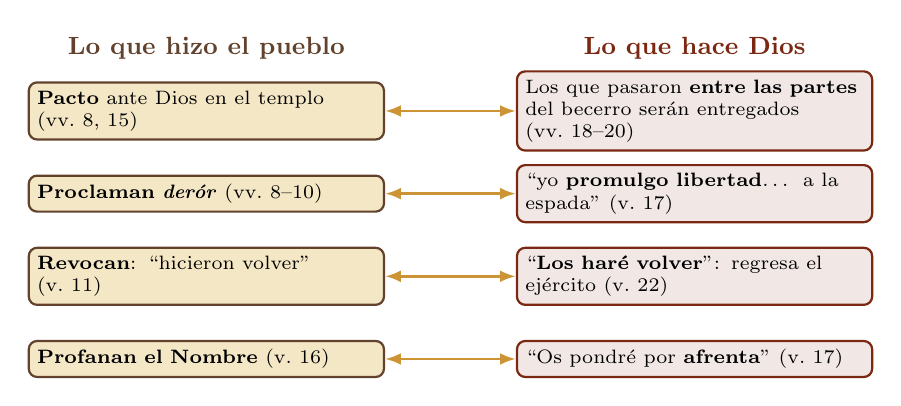
\begin{tikzpicture}[font=\scriptsize,
  izq/.style={caja,draw=sepia,text width=4.3cm,align=left,inner sep=3pt},
  der/.style={caja,fill=tierraroja!12,text width=4.3cm,align=left,inner sep=3pt}]
 \node[font=\small\bfseries,text=sepia] at (0,3.4) {Lo que hizo el pueblo};
 \node[font=\small\bfseries,text=tierraroja] at (6.2,3.4) {Lo que hace Dios};
 \node[izq] (a1) at (0,2.6) {\textbf{Pacto} ante Dios en el templo (vv.~8, 15)};
 \node[izq] (a2) at (0,1.55) {\textbf{Proclaman \emph{derór}} (vv.~8--10)};
 \node[izq] (a3) at (0,0.5) {\textbf{Revocan}: ``hicieron volver'' (v.~11)};
 \node[izq] (a4) at (0,-0.55) {\textbf{Profanan el Nombre} (v.~16)};
 \node[der] (b1) at (6.2,2.6) {Los que pasaron \textbf{entre las partes} del becerro serán entregados (vv.~18--20)};
 \node[der] (b2) at (6.2,1.55) {``yo \textbf{promulgo libertad}\ldots{} a la espada'' (v.~17)};
 \node[der] (b3) at (6.2,0.5) {``\textbf{Los haré volver}'': regresa el ejército (v.~22)};
 \node[der] (b4) at (6.2,-0.55) {``Os pondré por \textbf{afrenta}'' (v.~17)};
 \foreach \i in {1,2,3,4}{\draw[{Latex[length=2mm]}-{Latex[length=2mm]},mostaza!90!tierraroja,line width=1pt] (a\i.east) -- (b\i.west);}
\end{tikzpicture}\par\medskip
\scriptsize\RaggedRight El mismo verbo \emph{shuv} (``hacer volver'') en v.~11 y v.~22; \emph{derór} cuatro veces en el relato (conteo propio por lema).
\end{frame}

\begin{frame}{Tres ámbitos, un fundamento}
\centering
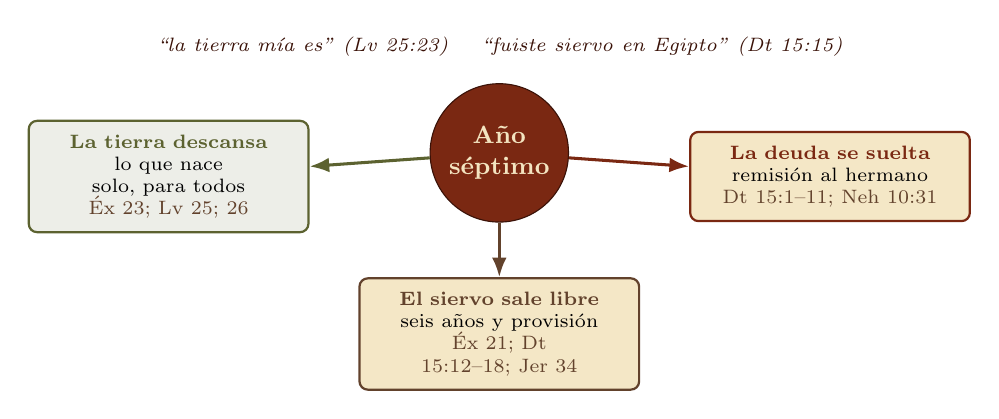
\begin{tikzpicture}[font=\scriptsize]
 \node[circle,fill=tierraroja,text=papiro,draw=caferojizo,minimum size=1.6cm,align=center,font=\small\bfseries] (c) at (0,0) {Año\\séptimo};
 \node[caja,draw=oliva,fill=oliva!12,text width=3.2cm,align=center] (t) at (-4.2,-0.3) {\textbf{\color{oliva}La tierra descansa}\\ lo que nace solo, para todos\\{\color{sepia}Éx 23; Lv 25; 26}};
 \node[caja,draw=sepia,text width=3.2cm,align=center] (s) at (0,-2.3) {\textbf{\color{sepia}El siervo sale libre}\\ seis años y provisión\\{\color{sepia}Éx 21; Dt 15:12--18; Jer 34}};
 \node[caja,text width=3.2cm,align=center] (d) at (4.2,-0.3) {\textbf{\color{tierraroja}La deuda se suelta}\\ remisión al hermano\\{\color{sepia}Dt 15:1--11; Neh 10:31}};
 \draw[-{Latex[length=2.5mm]},line width=1.1pt,oliva] (c) -- (t);
 \draw[-{Latex[length=2.5mm]},line width=1.1pt,sepia] (c) -- (s);
 \draw[-{Latex[length=2.5mm]},line width=1.1pt,tierraroja] (c) -- (d);
 \node[align=center,font=\scriptsize\itshape,text=caferojizo] at (0,1.35) {``la tierra mía es'' (Lv 25:23) \quad ``fuiste siervo en Egipto'' (Dt 15:15)};
\end{tikzpicture}
\end{frame}

\begin{frame}{Tabla sinóptica}
\fontsize{6.3}{7.5}\selectfont\renewcommand{\arraystretch}{1.1}
\begin{tabular}{@{}L{1.9cm}L{1.3cm}L{5.6cm}L{3.1cm}@{}}
\toprule
\textbf{Texto} & \textbf{Ámbito} & \textbf{Qué añade} & \textbf{Motivación} \\ \midrule
Éx 21:2--6 & siervo & seis años; ``libre, de balde''; oreja horadada & ley de casos \\
Éx 23:10--11 & tierra & tierra ``soltada'' y ``abandonada''; viñas y olivos & los pobres y las bestias \\
Lv 25:1--7 & tierra & \emph{shabat shabatón}; no sembrar ni podar; \emph{sefiaj} para todos & sábado del \SENOR{} \\
Lv 25:18--22 & tierra & ``¿qué comeremos?''; cosecha triple & la bendición mandada \\
Lv 26:34--43 & tierra & el exilio cobra los sábados & la desobediencia \\
Dt 15:1--11 & deudas & remisión pregonada; vv.~4/11; ``de Belial'' & ``no haya en medio de ti mendigo'' \\
Dt 15:12--18 & siervo & la hebrea; ``tu hermano''; provisión & ``fuiste siervo'' \\
Dt 31:9--13 & culto & la Torá leída en Sukkot (\emph{haqhel}) & oír, aprender, temer \\
Jer 34:8--22 & siervo & \emph{derór} proclamado y revocado & el pacto con los padres \\
2 Cr 36:20--21 & tierra & setenta años de reposo & la palabra de Jeremías \\
Neh 10:31 [10:32] & tierra, deudas & pacto que une Éx 23 y Dt 15 & renovación del pacto \\
\bottomrule
\end{tabular}
\end{frame}

% ------------------------------------------------------------------
\section{Historia}

\begin{frame}{Deuda y servidumbre}
\begin{columns}[t,onlytextwidth]
\begin{column}{0.50\textwidth}\small
\begin{itemize}
\item Mala cosecha $\rightarrow$ préstamo $\rightarrow$ prenda $\rightarrow$ tierra o hijos al acreedor.
\item ``Ha venido el acreedor para tomarse dos hijos míos por siervos'' (2 R 4:1).
\item ``Vendieron\ldots{} al pobre por un par de zapatos'' (Am 2:6).
\item Neh 5:1--13: tierras empeñadas, hijas en servidumbre; Nehemías obliga a devolver.
\end{itemize}
\end{column}
\begin{column}{0.48\textwidth}\small
\begin{itemize}
\item Edictos babilonios de \destacar{\emph{mīšarum}}: Ammi-saduqa (s.~\textsc{xvii} a.\,e.\,c.) anula deudas de consumo y libera a los entregados por deudas.
\item Acadio \emph{andurārum} $\approx$ hebreo \heb{דְּרוֹר}.
\item Hammurabi §117: servidumbre por deudas de tres años.
\end{itemize}
\precision{paralelos reales, pero el edicto era real e irregular; la shemitá es \emph{periódica}, \emph{divina} y da sábado a la \emph{tierra} (Weinfeld, 1995; Chirichigno, 1993).}
\end{column}
\end{columns}
\end{frame}

\begin{frame}{Una práctica atestiguada}
\centering
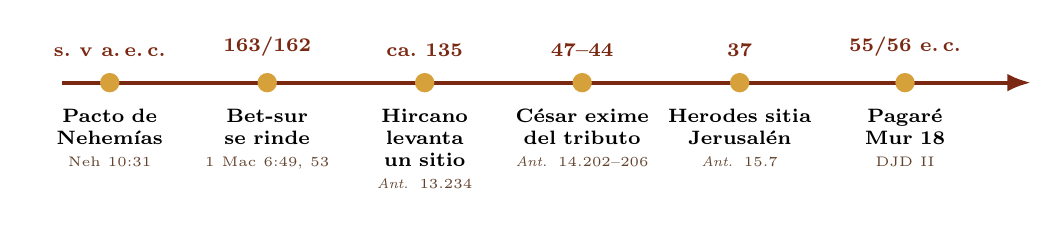
\begin{tikzpicture}[font=\scriptsize,x=1cm]
 \draw[line width=1.4pt,tierraroja,-{Latex[length=3mm]}] (0,0) -- (12.3,0);
 \foreach \x/\a/\b/\r in {0.6/{s.~\textsc{v} a.\,e.\,c.}/{Pacto de Nehemías}/{Neh 10:31},2.6/{163/162}/{Bet-sur se rinde}/{1 Mac 6:49, 53},4.6/{ca.~135}/{Hircano levanta un sitio}/{\emph{Ant.} 13.234},6.6/{47--44}/{César exime del tributo}/{\emph{Ant.} 14.202--206},8.6/{37}/{Herodes sitia Jerusalén}/{\emph{Ant.} 15.7},10.7/{55/56 e.\,c.}/{Pagaré Mur 18}/{DJD II}}{
   \fill[mostaza] (\x,0) circle (3.5pt);
   \node[above=6pt,font=\scriptsize\bfseries,text=tierraroja] at (\x,0) {\a};
   \node[below=6pt,text width=1.85cm,align=center] at (\x,0) {\textbf{\b}\\{\color{sepia}\tiny\r}};}
\end{tikzpicture}\par\medskip
\small\RaggedRight Tácito, \emph{Historias} 5.4: ``seducidos por la inercia'', dieron a la ociosidad también \destacar{el séptimo año} (trad. propia): prejuicio romano que confirma la práctica.\par\smallskip
\precision{la concesión de Alejandro (\emph{Ant.} 11.338) es relato legendario; la lectura condicional de Mur 18 (Milik, ``aunque sea año sabático'') está discutida; las fechas sabáticas varían en un año (Wacholder, 1973).}
\end{frame}

\begin{frame}{Qumrán y el décimo jubileo}
\begin{columns}[c,onlytextwidth]
\begin{column}{0.55\textwidth}\small
\begin{itemize}
\item 4Q319 (\emph{Otot}): el tiempo contado por \destacar{shemitot} y jubileos (VanderKam, 1998).
\item 11Q13 (Melquisedec): lee juntos \destacar{Lv 25:13, Dt 15:2 e Is 61:1}; Melquisedec proclama libertad en el décimo jubileo.
\item Es el antecedente judío más claro de Lc 4:18.
\end{itemize}
\end{column}
\begin{column}{0.43\textwidth}
\begin{cita}a publicar libertad a los cautivos, y a los presos apertura de la cárcel; a proclamar el año de la buena voluntad de \SENOR\ldots\fuente{(Is 61:1--2)}\end{cita}
\scriptsize\precision{texto de 11Q13 según García Martínez (1992) y Bergsma (2007).}
\end{column}
\end{columns}
\end{frame}

\begin{frame}{El exilio y los setenta años}
\centering
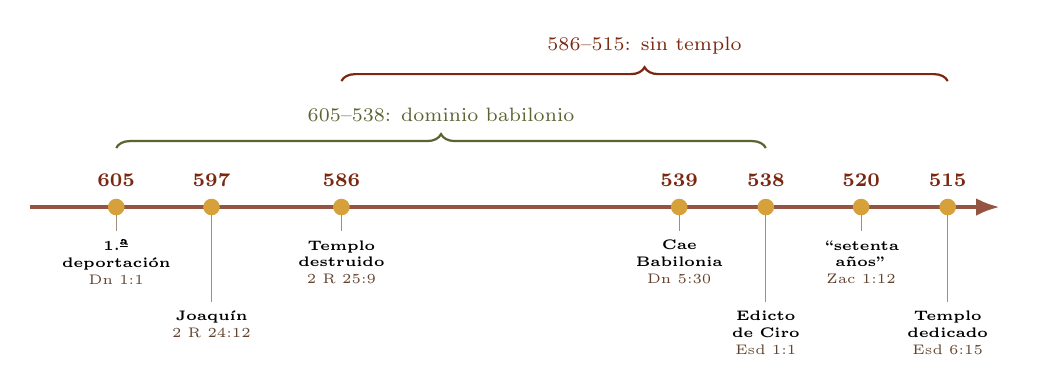
\begin{tikzpicture}[font=\scriptsize,x=0.11cm]
 \draw[line width=1.4pt,tierraroja!80,-{Latex[length=3mm]}] (0,0) -- (112,0);
 \foreach \a/\x in {605/10,597/21,586/36,539/75,538/85,520/96,515/106}{
   \fill[mostaza] (\x,0) circle (3pt);
   \node[above=4pt,font=\scriptsize\bfseries,text=tierraroja] at (\x,0) {\a};}
 \foreach \x/\t/\r/\y in {10/{1.ª deportación}/{Dn 1:1}/-0.3,21/{Joaquín}/{2 R 24:12}/-1.2,36/{Templo destruido}/{2 R 25:9}/-0.3,75/{Cae Babilonia}/{Dn 5:30}/-0.3,85/{Edicto de Ciro}/{Esd 1:1}/-1.2,96/{``setenta años''}/{Zac 1:12}/-0.3,106/{Templo dedicado}/{Esd 6:15}/-1.2}{
   \draw[sepia!60] (\x,-0.1) -- (\x,\y);
   \node[below,text width=1.6cm,align=center,font=\tiny] at (\x,\y) {\textbf{\t}\\{\color{sepia}\r}};}
 \draw[decorate,decoration={brace,amplitude=5pt},oliva,line width=0.8pt] (10,0.75) -- (85,0.75) node[midway,above=6pt,text=oliva] {605--538: dominio babilonio};
 \draw[decorate,decoration={brace,amplitude=5pt},tierraroja,line width=0.8pt] (36,1.6) -- (106,1.6) node[midway,above=6pt,text=tierraroja] {586--515: sin templo};
\end{tikzpicture}\par\medskip
\scriptsize\RaggedRight Tres lecturas: desde el dominio babilonio (Jer 25:11--12; Esd 1:1); desde la destrucción del templo (Zac 1:12; 7:5); número redondo de una vida (Sal 90:10).\par
\precision{fechas a.\,e.\,c. aproximadas. ``70 sábados incumplidos $=$ 490 años'' es lectura tradicional; Rashi (a Lv 26:35) calcula de otro modo con Ez 4:5--6 y los jubileos. El texto no hace la aritmética.}
\end{frame}

% ------------------------------------------------------------------
\section{Filología}

\begin{frame}{\heb{שׁמט} \emph{shamat}: soltar, dejar caer}
\begin{columns}[t,onlytextwidth]
\begin{column}{0.56\textwidth}
\scriptsize\renewcommand{\arraystretch}{1.12}
\begin{tabular}{@{}L{2.0cm}L{1.4cm}L{3.2cm}@{}}
\toprule
\textbf{Forma} & \textbf{Texto} & \textbf{Uso} \\ \midrule
\heb{שָׁמְטוּ הַבָּקָר} & 2 S 6:6 & los bueyes ``tropezaban'' \\
\heb{שִׁמְטֻהוּ} & 2 R 9:33 & ``echadla abajo'' (Jezabel) \\
\heb{נִשְׁמְטוּ} & Sal 141:6 & ``sean despeñados'' \\
\heb{תִּשְׁמְטֶנָּה} & Éx 23:11 & ``la soltarás'' (la tierra) \\
\heb{שָׁמוֹט} & Dt 15:2 & ``soltar'' la deuda \\
\heb{שְׁמִטָּה} & Dt 15:1, 2, 9; 31:10 & ``suelta, remisión'' \\
\bottomrule
\end{tabular}
\end{column}
\begin{column}{0.42\textwidth}\small
\begin{itemize}
\item La imagen de fondo es la de una \destacar{mano que suelta} lo que tenía agarrado.
\item \emph{Shemitá}: solo en Deuteronomio, 5 veces (conteo propio por lema).
\item LXX: \grc{ἀφίημι}, \grc{ἄφεσις}.
\end{itemize}
\end{column}
\end{columns}
\end{frame}

\begin{frame}{\emph{Shabatón}, \emph{sefiaj}, \emph{nazir}}
\scriptsize\renewcommand{\arraystretch}{1.18}
\begin{tabular}{@{}L{2.5cm}L{2.0cm}L{7.4cm}@{}}
\toprule
\textbf{Palabra} & \textbf{Texto} & \textbf{Sentido} \\ \midrule
\heb{שַׁבַּת שַׁבָּתוֹן} & Lv 25:4 & ``sábado de reposo solemne'': superlativo; mismo título que el sábado (Lv 23:3) y Yom Kipur (16:31). \\
\heb{שַׁבְּתֹתֶיהָ} & Lv 26:34; 2 Cr 36:21 & ``sus sábados'': la tierra los ``goza'' en el exilio. \\
\heb{סְפִיחַ} \emph{sefiaj} & Lv 25:5; 2 R 19:29 & lo que brota solo del grano caído; Israel come como en el Edén. \\
\heb{עִנְּבֵי נְזִירֶךָ} & Lv 25:5 & ``uvas de tu \emph{nazir}'': la vid no podada, como el cabello del \destacar{nazareo} (Nm 6:5). RVR1960: ``tu viñedo''. \\
\heb{אֶבְיוֹן}, \heb{עָנִי} & Éx 23:11; Dt 15:4, 11 & el que depende de otro; el abajado. ``\emph{Tu} pobre'' (Dt 15:11). \\
\heb{נָשָׁה} & Dt 15:2; 2 R 4:1 & prestar, ser acreedor: \heb{בַּעַל מַשֵּׁה יָדוֹ}; \heb{הַנֹּשֶׁה}, ``el acreedor''. \\
\bottomrule
\end{tabular}\par\medskip
\precision{el juego \emph{nazir} / nazareato es señalado por Milgrom (2001) y Hartley (1992).}
\end{frame}

\begin{frame}{\heb{דְּרוֹר} \emph{derór}: la libertad que se proclama}
\begin{columns}[c,onlytextwidth]
\begin{column}{0.36\textwidth}
\centering
\begin{tikzpicture}
 \node[circle,fill=tierraroja,text=papiro,minimum size=1.7cm,font=\Large] (d) {\heb{דְּרוֹר}};
 \node[caja,above=0.35cm of d,text width=2.6cm,align=center] {siempre se \textbf{proclama} (\emph{qará})};
 \node[caja,below=0.35cm of d,text width=2.6cm,align=center] {acadio \emph{andurārum}};
\end{tikzpicture}
\end{column}
\begin{column}{0.62\textwidth}\small
\begin{itemize}
\item Lv 25:10: ``pregonaréis \destacar{libertad} en la tierra'' (jubileo).
\item Jer 34:8, 15, 17: la libertad de Sedequías y la ``libertad a la espada''.
\item Is 61:1: ``publicar libertad a los cautivos''.
\item Ez 46:17: \emph{shnat haderór}, ``el año de la libertad'' (RVR1960: ``del jubileo'').
\item Sal 84:3 [84:4]: \emph{derór}, ``la golondrina'', el ave libre.
\item LXX: \grc{ἄφεσις} en Lv 25:10 e Is 61:1.
\end{itemize}
\end{column}
\end{columns}
\end{frame}

\begin{frame}{Del hebreo al perdón}
\centering
\resizebox{\linewidth}{!}{%
\begin{tikzpicture}[font=\scriptsize,node distance=0.5cm]
 \node[caja,text width=3.0cm,align=center] (h) {\textbf{Hebreo}\\[2pt] \heb{שְׁמִטָּה} (Éx 23:11; Dt 15:1--2)\\[2pt] \heb{דְּרוֹר} (Lv 25:10; Is 61:1)};
 \node[caja,text width=3.0cm,align=center,right=of h] (l) {\textbf{Septuaginta}\\[2pt] \grc{ἄφεσις}, \grc{ἀφίημι}\\ ``suelta, soltar''\\ \grc{χρέος}, \grc{ὀφείλω}: ``deuda''};
 \node[draw=mostaza,line width=1.5pt,fill=tierraroja,text=papiro,rounded corners=3pt,text width=3.2cm,align=center,inner sep=5pt,right=of l] (n) {\textbf{Nuevo Testamento}\\[2pt] \grc{ἄφεσιν} (Lc 4:18)\\ \grc{ἄφες\ldots\ ὀφειλήματα} (Mt 6:12)\\ \grc{εἰς ἄφεσιν ἁμαρτιῶν} (Mt 26:28)};
 \node[caja,fill=white,text width=2.3cm,align=center,right=of n] (e) {\textbf{RVR1960}\\[2pt] ``remisión''\\ ``libertad''\\ ``perdón''};
 \draw[-{Latex[length=3mm]},mostaza!90!tierraroja,line width=1.3pt] (h)--(l);
 \draw[-{Latex[length=3mm]},mostaza!90!tierraroja,line width=1.3pt] (l)--(n);
 \draw[-{Latex[length=3mm]},mostaza!90!tierraroja,line width=1.3pt] (n)--(e);
\end{tikzpicture}}\par\medskip
\small\RaggedRight En griego, la tierra soltada, la deuda remitida y el cautivo liberado se dicen \destacar{con la misma palabra} que el perdón de los pecados.
\end{frame}

\begin{frame}{\grc{ἄφεσις} en la Septuaginta}
\scriptsize\renewcommand{\arraystretch}{1.18}
\begin{tabular}{@{}L{1.8cm}L{3.3cm}L{4.0cm}L{2.8cm}@{}}
\toprule
\textbf{Texto} & \textbf{Hebreo} & \textbf{LXX} & \textbf{Sentido} \\ \midrule
Éx 23:11 & \heb{תִּשְׁמְטֶנָּה} & \grc{ἄφεσιν ποιήσεις} & soltar la tierra \\
Dt 15:1 & \heb{תַּעֲשֶׂה שְׁמִטָּה} & \grc{ποιήσεις ἄφεσιν} & hacer remisión \\
Dt 15:2 & \heb{שָׁמוֹט} & \grc{ἀφήσεις πᾶν χρέος ἴδιον} & soltar toda deuda \\
Lv 25:10 & \heb{וּקְרָאתֶם דְּרוֹר} & \grc{διαβοήσετε ἄφεσιν} & pregonar libertad \\
Lv 25:10 & \heb{יוֹבֵל} & \grc{ἐνιαυτὸς ἀφέσεως σημασία} & ``año de la suelta'' \\
Is 61:1 & \heb{לִשְׁבוּיִם דְּרוֹר} & \grc{αἰχμαλώτοις ἄφεσιν} & libertad a cautivos \\
\bottomrule
\end{tabular}\par\medskip
\precision{en el NT, \grc{ἄφεσις} es ante todo ``perdón'' (BDAG). La resonancia de la shemitá es mayor en Lc 4:18 y Mt 6:12; 18:23--35 que en Hch 2:38.}
\end{frame}

\begin{frame}{``Perdónanos nuestras deudas''}
\fotolado{panel_mateo6.jpg}{Elaboración propia: Mt 6:12 en escritura uncial (texto NA28).}
\begin{columns}[c,onlytextwidth]
\begin{column}{0.57\textwidth}
\begin{cita}Y perdónanos nuestras deudas, como también nosotros perdonamos a nuestros deudores.\fuente{(Mt 6:12, RVR1960)}\end{cita}
\scriptsize \grc{ἄφες ἡμῖν τὰ ὀφειλήματα ἡμῶν}: vocabulario de Dt 15:2 LXX (\grc{ἀφήσεις\ldots\ ὀφείλει}). Lc 11:4: ``pecados'', pero ``a todos los que \destacar{nos deben}''.\par\smallskip
Mt 18:23--35: el rey ``le perdonó la deuda'' (\grc{τὸ δάνειον ἀφῆκεν}); el siervo no suelta a su consiervo, como un \destacar{Dt 15 narrado}.
\end{column}
\begin{column}{0.41\textwidth}\end{column}
\end{columns}
\end{frame}

% ------------------------------------------------------------------
\section{Texto}

\begin{frame}{Cuestiones textuales}
\begin{columns}[t,onlytextwidth]
\begin{column}{0.49\textwidth}\scriptsize
\textbf{\color{tierraroja}Dt 15:2}: \heb{שָׁמוֹט כָּל־בַּעַל מַשֵּׁה יָדוֹ אֲשֶׁר יַשֶּׁה בְּרֵעֵהוּ}\\
(a) ``todo acreedor soltará lo que prestó'' (Tigay, 1996); (b) suelta ``la prenda''. ¿Cancelación o suspensión? v.~2b y v.~9 favorecen \destacar{cancelación} (Hamilton, 1992). LXX: \grc{ἀφήσεις πᾶν χρέος}.\par\medskip
\textbf{\color{tierraroja}Lv 25:5--6}: prohíbe \emph{segar} y \emph{vendimiar} (cosecha organizada), no \emph{comer} del campo (Milgrom, 2001).
\end{column}
\begin{column}{0.49\textwidth}\scriptsize
\textbf{\color{tierraroja}2 Cr 36:21}: cita compuesta: Jeremías (70 años) + Lv 26:34--35 (sábados), atribuida al profeta.\par\medskip
\textbf{\color{tierraroja}Dt 15:18}: \heb{מִשְׁנֶה שְׂכַר שָׂכִיר}, ``el doble'' o ``el equivalente'' del jornal; RVR1960 ``la mitad del costo''.\par\medskip
\begin{tcolorbox}[colback=mostaza!12,colframe=mostaza!85!tierraroja,boxrule=0.6pt,arc=2pt,left=3pt,right=3pt,top=2pt,bottom=2pt,title=Precisión textual,fonttitle=\bfseries\scriptsize,coltitle=caferojizo,colbacktitle=mostaza!30]
\heb{מִקֵּץ שֶׁבַע שָׁנִים} = ``al llegar el séptimo'' (cf. Jer 34:14: ``le servirá seis años''). La RVR1960 pierde el juego \emph{nazir}.
\end{tcolorbox}
\end{column}
\end{columns}
\end{frame}

% ------------------------------------------------------------------
\section{Literatura}

\begin{frame}{La escalera del siete}
\centering
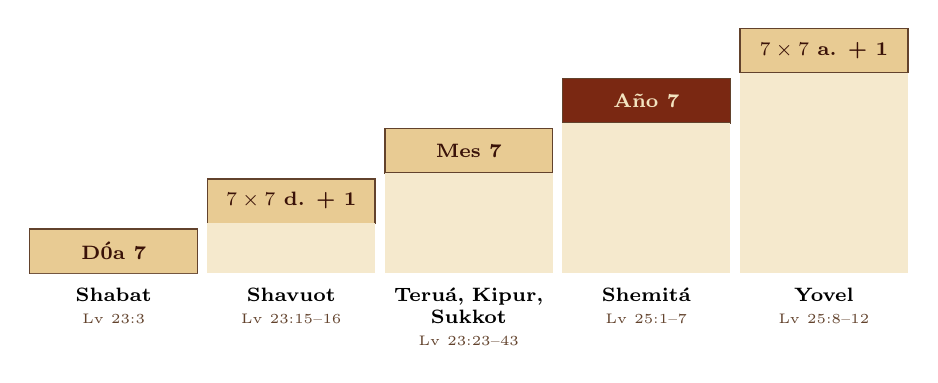
\begin{tikzpicture}[font=\scriptsize,x=0.82cm,y=0.75cm]
 \foreach \i/\t/\d/\r in {0/{Día 7}/{Shabat}/{Lv 23:3},1/{$7\times7$ d. + 1}/{Shavuot}/{Lv 23:15--16},2/{Mes 7}/{Teruá, Kipur, Sukkot}/{Lv 23:23--43},3/{Año 7}/{Shemitá}/{Lv 25:1--7},4/{$7\times7$ a. + 1}/{Yovel}/{Lv 25:8--12}}{
   \pgfmathsetmacro{\x}{\i*2.75}
   \pgfmathsetmacro{\y}{\i*0.85}
   \ifnum\i=3
     \fill[tierraroja] (\x,\y) rectangle ++(2.6,0.75);
     \node[text=papiro,font=\scriptsize\bfseries] at (\x+1.3,\y+0.38) {\t};
   \else
     \fill[mostaza!55] (\x,\y) rectangle ++(2.6,0.75);
     \node[text=caferojizo,font=\scriptsize\bfseries] at (\x+1.3,\y+0.38) {\t};
   \fi
   \draw[sepia,line width=0.5pt] (\x,\y) rectangle ++(2.6,0.75);
   \fill[papiro!80] (\x,0) rectangle ++(2.6,\y);
   \node[anchor=north,text width=1.95cm,align=center] at (\x+1.3,-0.08) {\textbf{\d}\\{\color{sepia}\tiny \r}};}
\end{tikzpicture}\par\medskip
\small\RaggedRight Las dos series paralelas, de días y de años, desembocan en un \destacar{``cincuenta''}: Shavuot y el jubileo. Cada escalón amplía el alcance del reposo.
\end{frame}

\begin{frame}{Siete sábados de años}
\begin{columns}[c,onlytextwidth]
\begin{column}{0.62\textwidth}
\centering
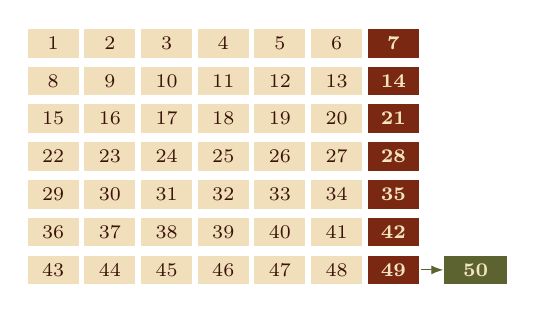
\begin{tikzpicture}[font=\scriptsize,x=0.72cm,y=0.48cm]
 \foreach \r in {1,...,7}{
   \foreach \c in {1,...,7}{
     \pgfmathtruncatemacro{\n}{(\r-1)*7+\c}
     \ifnum\c=7
       \fill[tierraroja] (\c-0.45,-\r+0.62) rectangle (\c+0.45,-\r+1.38);
       \node[text=papiro,font=\scriptsize\bfseries] at (\c,-\r+1) {\n};
     \else
       \fill[mostaza!35] (\c-0.45,-\r+0.62) rectangle (\c+0.45,-\r+1.38);
       \node[text=caferojizo] at (\c,-\r+1) {\n};
     \fi}}
 \fill[oliva] (7.9,-6.38) rectangle (9.0,-5.62);
 \node[text=papiro,font=\scriptsize\bfseries] at (8.45,-6) {50};
 \draw[-{Latex[length=1.5mm]},oliva] (7.48,-6) -- (7.88,-6);
\end{tikzpicture}
\end{column}
\begin{column}{0.36\textwidth}\small\RaggedRight
\heb{שֶׁבַע שַׁבְּתֹת שָׁנִים}: ``siete \destacar{sábados} de años'' (Lv 25:8).\par\medskip
\textcolor{tierraroja}{\rule{2mm}{2mm}} shemitá: 7, 14\ldots{} 49\\
\textcolor{oliva}{\rule{2mm}{2mm}} yovel: año 50, en Yom Kipur (25:9)\par\medskip
\precision{si el 50 es también el año 1 del ciclo siguiente se discute (cap. 09).}
\end{column}
\end{columns}
\end{frame}

\begin{frame}{Lv 25 en la síntesis de la serie}
\begin{columns}[c,onlytextwidth]
\begin{column}{0.60\textwidth}
\centering
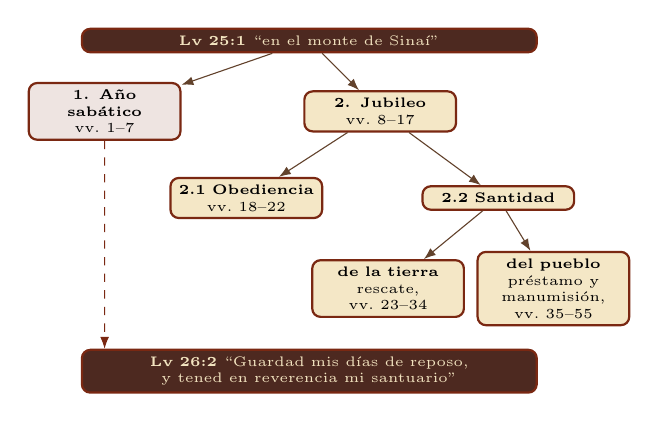
\begin{tikzpicture}[font=\tiny,
  bl/.style={caja,font=\tiny,text width=1.75cm,align=center,inner sep=2.5pt},
  rj/.style={caja,font=\tiny,fill=tierraroja!14,text width=1.75cm,align=center,inner sep=2.5pt}]
 \node[caja,font=\tiny,fill=caferojizo,text=papiro,text width=5.6cm,align=center,inner sep=2.5pt] (s) at (0,0) {\textbf{Lv 25:1} ``en el monte de Sinaí''};
 \node[rj] (a) at (-2.6,-0.9) {\textbf{1. Año sabático}\\ vv.~1--7};
 \node[bl] (b) at (0.9,-0.9) {\textbf{2. Jubileo}\\ vv.~8--17};
 \node[bl] (b1) at (-0.8,-2.0) {\textbf{2.1 Obediencia}\\ vv.~18--22};
 \node[bl] (b2) at (2.4,-2.0) {\textbf{2.2 Santidad}};
 \node[bl] (t) at (1.0,-3.15) {\textbf{de la tierra}\\ rescate, vv.~23--34};
 \node[bl] (p) at (3.1,-3.15) {\textbf{del pueblo}\\ préstamo y manumisión, vv.~35--55};
 \node[caja,font=\tiny,fill=caferojizo,text=papiro,text width=5.6cm,align=center,inner sep=2.5pt] (c) at (0,-4.2) {\textbf{Lv 26:2} ``Guardad mis días de reposo, y tened en reverencia mi santuario''};
 \draw[-{Latex[length=1.5mm]},sepia] (s) -- (a); \draw[-{Latex[length=1.5mm]},sepia] (s) -- (b);
 \draw[-{Latex[length=1.5mm]},sepia] (b) -- (b1); \draw[-{Latex[length=1.5mm]},sepia] (b) -- (b2);
 \draw[-{Latex[length=1.5mm]},sepia] (b2) -- (t); \draw[-{Latex[length=1.5mm]},sepia] (b2) -- (p);
 \draw[-{Latex[length=1.5mm]},tierraroja,dashed] (a.south) -- ([xshift=-2.6cm]c.north);
\end{tikzpicture}
\end{column}
\begin{column}{0.38\textwidth}\scriptsize\RaggedRight
\begin{itemize}
\item ``La tierra mía es'' (v.~23); el pariente rescata (v.~25).
\item No explotarse; obrar con temor de Dios (vv.~14--17).
\item Préstamo sin interés; el hermano sirve como jornalero, no como esclavo (vv.~35--43).
\item Lv 25:1 y 26:46: \destacar{inclusión sinaítica}; ``siete veces más'' (26:18--28).
\end{itemize}
{\fontsize{5}{6}\selectfont\color{sepia}\textit{Nota.} Elaboración propia a partir de la presentación \emph{El Jubileo} de la serie.}
\end{column}
\end{columns}
\end{frame}

\begin{frame}{Daniel 9: setenta heptadas}
\begin{cita}Setenta semanas están determinadas sobre tu pueblo y sobre tu santa ciudad\ldots\fuente{(Dn 9:24)}\end{cita}
\centering
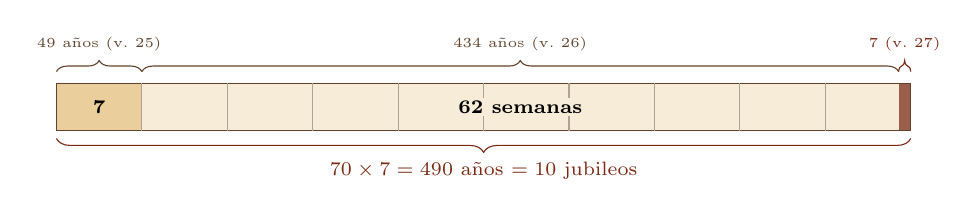
\begin{tikzpicture}[font=\scriptsize,x=0.155cm]
 \fill[mostaza!50] (0,0) rectangle (7,0.6);
 \fill[mostaza!20] (7,0) rectangle (69,0.6);
 \fill[tierraroja!75] (69,0) rectangle (70,0.6);
 \draw[sepia] (0,0) rectangle (70,0.6);
 \foreach \x in {7,14,...,63}{\draw[sepia!50] (\x,0) -- (\x,0.6);}
 \node[font=\scriptsize\bfseries] at (3.5,0.3) {7};
 \node[font=\scriptsize\bfseries,fill=mostaza!20,inner sep=1pt] at (38,0.3) {62 semanas};
 \draw[decorate,decoration={brace,amplitude=4pt},sepia] (0,0.75) -- (7,0.75) node[midway,above=4pt,font=\tiny] {49 años (v.~25)};
 \draw[decorate,decoration={brace,amplitude=4pt},sepia] (7,0.75) -- (69,0.75) node[midway,above=4pt,font=\tiny] {434 años (v.~26)};
 \draw[decorate,decoration={brace,amplitude=4pt},tierraroja] (69,0.75) -- (70,0.75) node[midway,above=4pt,font=\tiny,text=tierraroja] {7 (v.~27)};
 \draw[decorate,decoration={brace,amplitude=5pt,mirror},tierraroja] (0,-0.1) -- (70,-0.1) node[midway,below=5pt,text=tierraroja] {$70\times7=490$ años $=10$ jubileos};
\end{tikzpicture}\par\medskip
\scriptsize\RaggedRight Daniel relee los setenta años de Jeremías (Dn 9:2) con la aritmética sabática; cf. 11Q13, ``décimo jubileo''.\par
\precision{esquema interpretativo. Lecturas: mesiánica (decreto persa $\rightarrow$ Cristo), macabea (Collins, 1993), futurista (semana final futura). Cap. 09.}
\end{frame}

% ------------------------------------------------------------------
\section{La serie}

\begin{frame}{El reglamento del culto y el sábado}
\begin{columns}[c,onlytextwidth]
\begin{column}{0.52\textwidth}\small
\begin{itemize}
\item Lv 23 $=$ \destacar{reglamento del culto}: ``citaciones santas'' en sus tiempos, estatuto perpetuo.
\item Distinto de la ley de los sacrificios (Lv 1--7; Nm 28--29).
\item Primer renglón: el sábado, memorial de la creación, señal y ``símbolo de la vida eterna después del Milenio''.
\end{itemize}
\end{column}
\begin{column}{0.46\textwidth}
\begin{tcolorbox}[colback=papiro,colframe=tierraroja,boxrule=1pt,arc=3pt]
\small La shemitá no se celebra cada año: es el \destacar{sábado proyectado sobre los años}, con su mismo título y en el mismo Sinaí (Lv 25:1).
\end{tcolorbox}
\precision{la shemitá no es convocación de Lv 23; aquí se le aplica el marco de la serie.}
\end{column}
\end{columns}
\end{frame}

\begin{frame}{Memorial y figura}
\scriptsize\renewcommand{\arraystretch}{1.16}
\begin{tabular}{@{}L{3.3cm}L{3.3cm}L{5.4cm}@{}}
\toprule
\textbf{Hito de Israel} & \textbf{Shemitá} & \textbf{Nuevo Pacto (lectura de la serie)} \\ \midrule
Salida de Egipto: ``fuiste siervo'' (Dt 15:15) & el siervo sale libre y con provisión & libertad del pecado (Jn 8:34--36; Ro 6:22--23) \\
Entrada con Josué (Lv 25:2) & la tierra guarda sábado & ``queda un reposo'' (He 4:8--9) \\
Exilio (2 Cr 36:21) & los sábados cobrados & ``Si oyereis hoy su voz'' (He 3:7--4:7) \\
Remisión de deudas (Dt 15:1--2) & \grc{ἄφεσις} (LXX) & \grc{ἄφεσις ἁμαρτιῶν} (Mt 26:28) \\
Torá en Sukkot (Dt 31:10--13) & el pueblo liberado oye la ley & la ley en el corazón (Jer 31:33); Sukkot $=$ Milenio \\
Sábado de la creación (Gn 2:2--3) & la tierra imita a su Creador & la creación libertada (Ro 8:21; Ap 21:1) \\
\bottomrule
\end{tabular}\par\smallskip
\precision{la columna derecha es lectura tipológica de la serie.}
\end{frame}

\begin{frame}{El reposo que no se alcanzó con Josué}
\begin{columns}[c,onlytextwidth]
\begin{column}{0.52\textwidth}
\begin{cita}Porque si Josué les hubiera dado el reposo, no hablaría después de otro día. Por tanto, queda un reposo para el pueblo de Dios.\fuente{(He 4:8--9, RVR1960)}\end{cita}
\scriptsize \grc{σαββατισμός}: ``guarda de sábado''.
\end{column}
\begin{column}{0.46\textwidth}
\centering
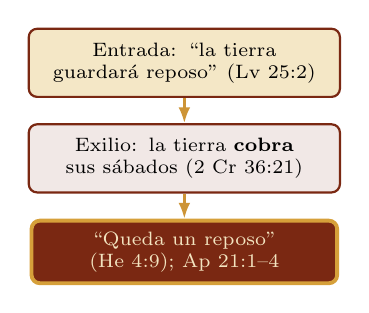
\begin{tikzpicture}[font=\scriptsize,node distance=0.32cm]
 \node[caja,text width=3.6cm,align=center] (a) {Entrada: ``la tierra guardará reposo'' (Lv 25:2)};
 \node[caja,fill=tierraroja!12,text width=3.6cm,align=center,below=of a] (b) {Exilio: la tierra \textbf{cobra} sus sábados (2 Cr 36:21)};
 \node[draw=mostaza,line width=1.4pt,fill=tierraroja,text=papiro,rounded corners=3pt,text width=3.6cm,align=center,inner sep=4pt,below=of b] (c) {``Queda un reposo'' (He 4:9); Ap 21:1--4};
 \draw[-{Latex[length=2mm]},mostaza!90!tierraroja,line width=1pt] (a)--(b);
 \draw[-{Latex[length=2mm]},mostaza!90!tierraroja,line width=1pt] (b)--(c);
\end{tikzpicture}
\end{column}
\end{columns}\medskip
\precision{Hebreos es anónima; la tradición antigua la atribuyó a menudo a Pablo (Attridge, 1989; Lane, 1991).}
\end{frame}

\begin{frame}{El sábado de los milenios}
\begin{columns}[t,onlytextwidth]
\begin{column}{0.52\textwidth}\small
\begin{itemize}
\item En el Milenio, Dios transformará hasta la naturaleza de los animales salvajes (Is 11:6--9).
\item ``Seis mil años'' y ``mil años de descanso'' (Baker, 2013).
\item Mi presentación anterior: ``casi 6,000 años y 120 jubileos''; la tierra ``alcanzará el reposo total''.
\end{itemize}
\end{column}
\begin{column}{0.46\textwidth}\small
\begin{itemize}
\item Talmud, \emph{Sanedrín} 97a (Rav Ketina): como la shemitá, el mundo descansa mil años de cada siete mil.
\item \emph{Bernabé} 15:4--5: seis días $=$ seis mil años.
\end{itemize}
\precision{Sal 90:4 y 2 P 3:8 no forman un calendario; la serie asocia el Milenio a Sukkot y el sábado a la eternidad: no confundir los dos mapas tipológicos.}
\end{column}
\end{columns}
\end{frame}

% ------------------------------------------------------------------
\section{Mesías}

\begin{frame}{Nazaret: ``el año agradable''}
\begin{columns}[c,onlytextwidth]
\begin{column}{0.55\textwidth}
\begin{cita}\ldots{}A pregonar libertad a los cautivos, Y vista a los ciegos; A poner en libertad a los oprimidos; A predicar el año agradable del Señor.\fuente{(Lc 4:18--19, RVR1960)}\end{cita}
\scriptsize Is 61:1--2 junto con Is 58:6 da \grc{ἄφεσις} \destacar{dos veces}. ``Hoy se ha cumplido esta Escritura'' (4:21).
\end{column}
\begin{column}{0.43\textwidth}\small
\begin{itemize}
\item Vocabulario del jubileo y de la remisión.
\item Antecedente: 11Q13.
\end{itemize}
\precision{¿jubileo literal? Yoder (1972) sí, con consecuencias económicas; Sloan (1977): teología jubilar escatológica de Lucas; otros: solo alusión a Isaías.}
\end{column}
\end{columns}
\end{frame}

\begin{frame}{``¿Qué comeremos?'' y ``ningún necesitado''}
\begin{columns}[t,onlytextwidth]
\begin{column}{0.49\textwidth}
\begin{cita}No os afanéis, pues, diciendo: ¿Qué comeremos, o qué beberemos\ldots? Mas buscad primeramente el reino de Dios y su justicia\ldots\fuente{(Mt 6:31--33)}\end{cita}
\scriptsize \grc{Τί φάγωμεν;} se hace eco de Lv 25:20 (\destacar{eco}, no cita).
\end{column}
\begin{column}{0.49\textwidth}
\begin{cita}Así que no había entre ellos ningún necesitado\ldots\fuente{(Hch 4:34)}\end{cita}
\scriptsize \grc{οὐδὲ γὰρ ἐνδεής τις ἦν} $\approx$ Dt 15:4 LXX \grc{οὐκ ἔσται ἐν σοὶ ἐνδεής}.\par
\precision{eco probable: \grc{ἐνδεής} solo aquí en el NT; compartir voluntario (Hch 5:4), no remisión periódica.}
\end{column}
\end{columns}
\end{frame}

\begin{frame}{Pablo: igualdad y creación libertada}
\begin{columns}[t,onlytextwidth]
\begin{column}{0.49\textwidth}
\begin{cita}\ldots{}para que haya igualdad, como está escrito: El que recogió mucho, no tuvo más, y el que poco, no tuvo menos.\fuente{(2 Co 8:14--15)}\end{cita}
\scriptsize \grc{ἰσότης}: la pedagogía del maná (Éx 16:18) y de Lv 25:20--22.
\end{column}
\begin{column}{0.49\textwidth}
\begin{cita}\ldots{}también la creación misma será libertada de la esclavitud de corrupción a la libertad gloriosa de los hijos de Dios.\fuente{(Ro 8:21)}\end{cita}
\scriptsize La tierra que ``gime'' aguarda su sábado (cf. Lv 26:42; Gn 3:17; Moo, 1996).
\end{column}
\end{columns}
\end{frame}

% ------------------------------------------------------------------
\section{Tradición}

\begin{frame}{Misná \emph{Sheviít} y el \emph{prosbul}}
\begin{columns}[c,onlytextwidth]
\begin{column}{0.54\textwidth}\small
\begin{itemize}
\item Tratado \emph{Sheviít} (orden \emph{Zeraim}): trabajos prohibidos, fruto sin dueño, remisión (cap. 10).
\item Hillel notó que se dejaba de prestar antes del año séptimo, contra Dt 15:9, e instituyó el \destacar{\emph{prosbul}}: la deuda pasa al tribunal (\emph{Sheviít} 10:3--4).
\item \emph{Haqhel}: el rey Agripa lee y llora en Dt 17:15 (\emph{Sotá} 7:8).
\item El exilio viene por no dejar descansar la tierra (\emph{Avot} 5:9).
\end{itemize}
\end{column}
\begin{column}{0.44\textwidth}\small
\begin{itemize}
\item Israel moderno: \emph{heter mejirá} (1888--1889; Rav Kook) u \emph{otsar bet din}.
\item Último año sabático: 5782 (2021--2022); el siguiente, 5789 (2028--2029).
\end{itemize}
\precision{todo es tradición rabínica o práctica moderna; \emph{Guitín} 36a: hoy, de autoridad rabínica.}
\end{column}
\end{columns}
\end{frame}

% ------------------------------------------------------------------
\section{Discusión}

\begin{frame}{¿Obliga hoy la shemitá?}
\begin{tikzpicture}
 \foreach \x/\y/\n/\t/\d in {0/0/1/{Judaísmo rabínico}/{solo en la tierra de Israel; hoy rabínica (Guitín 36a); \emph{prosbul}},6.0/0/2/{Principio ético}/{paradigma: tierra de Dios, deuda no perpetua, pobre hermano (Wright, 2004; Hamilton, 1992; Milgrom, 2001)},0/-2.15/3/{Cumplida en Cristo}/{ley civil y ceremonial; \grc{ἄφεσις} y reposo en Cristo (Mt 11:28; He 4)},6.0/-2.15/4/{Lectura de la serie}/{vigencia de Lv 23; año séptimo ligado a la tierra, principio vivo y figura del reposo final}}{
  \node[caja,anchor=north west] (b\n) at (\x,\y) {\parbox[t][1.45cm][t]{5.3cm}{\RaggedRight{\small\textbf{\textcolor{tierraroja}{\t}}}\\[2pt]\scriptsize \d}};
  \node[circle,fill=tierraroja,text=papiro,font=\scriptsize\bfseries,inner sep=1.6pt] at (b\n.north west) {\n};}
\end{tikzpicture}\par\medskip
\precision{las posturas no siempre se excluyen. Lo que el texto no permite es leer la shemitá solo como metáfora: sus destinatarios fueron campesinos, deudores y siervos reales (Jer 34).}
\end{frame}

% ------------------------------------------------------------------
\section{Síntesis}

\begin{frame}{Definición}
\begin{tcolorbox}[colback=papiro,colframe=tierraroja,boxrule=1pt,arc=3pt,fonttitle=\bfseries,title=Shemitá]
\small El año séptimo, en que ``la tierra tendrá descanso, reposo para \SENOR'' (Lv 25:4): la tierra no se siembra y lo que nace solo es para todos (Éx 23:10--11; Lv 25:5--7); el acreedor suelta la deuda del hermano (Dt 15:1--11); el siervo sale libre con provisión (Éx 21:2; Dt 15:12--18); la Torá se lee en Sukkot (Dt 31:10--13). Se funda en que la tierra es de Dios (Lv 25:23) y en la memoria de Egipto (Dt 15:15). Su incumplimiento fue exilio (2 Cr 36:21); su vocabulario, perdón (\grc{ἄφεσις}); su reposo, figura del sábado que queda (He 4:9).
\end{tcolorbox}
\end{frame}

\begin{frame}{Lectura $\rightarrow$ aporte}
\scriptsize\renewcommand{\arraystretch}{1.15}
\begin{tabular}{@{}L{2.3cm}L{9.7cm}@{}}
\toprule
\textbf{Lectura} & \textbf{Aporte} \\ \midrule
Textos & red de leyes: tierra, siervo, deudas, culto \\
Histórica & responde a deuda y servidumbre; \emph{mīšarum} transformado; práctica de Nehemías al siglo \textsc{i} \\
Filológica & \emph{shamat} ``soltar''; \emph{nazir}; \emph{derór}; LXX \grc{ἄφεσις} $\rightarrow$ perdón \\
Textual & Dt 15:2: cancelación; Lv 25:5--6: cosechar $\neq$ comer; 2 Cr 36:21 compuesta \\
Literaria & escalera del siete; Lv 25--26 sinaítico; ``siete veces más''; Dn 9 \\
La serie & prolonga el sábado de Lv 23:3; memoria del éxodo y de Josué; reposo que queda \\
NT & Lc 4:18; Mt 6:12; 18:23--35; 6:31; Hch 4:34; 2 Co 8:13--15; Ro 8:21; He 4:9 \\
\bottomrule
\end{tabular}\par\medskip
\small\RaggedRight La tierra guardó por fuerza los sábados que el pueblo no quiso darle. De esa paradoja viene la esperanza de un reposo que dependa del Dios que \destacar{manda su bendición} y \destacar{remite las deudas}.
\end{frame}

% ------------------------------------------------------------------
\section{Reflexión}

\begin{frame}{Para la reflexión}
\small
\begin{enumerate}
\item ¿Qué decisiones económicas se toman por miedo a ``¿qué comeremos?'' (Lv 25:20; Mt 6:33)?
\item ¿Dónde aparece hoy el ``pensamiento de Belial'' que deja de ayudar porque no conviene (Dt 15:9)?
\item ¿Qué deudas habría que ``soltar'' a un hermano (Mt 6:12; 18:23--35)?
\item ¿Cómo acompañar a quien sale de una dependencia ``con las manos llenas'' (Dt 15:13--14)?
\item ¿Qué promesas hechas en la crisis se revocan cuando la crisis pasa (Jer 34)?
\item ¿Qué lugar tiene la lectura completa y comunitaria de la Escritura (Dt 31:10--13)?
\end{enumerate}
\end{frame}

% ------------------------------------------------------------------
\section{Glosario}

\begin{frame}{Glosario}
\fontsize{6.6}{7.8}\selectfont
\begin{columns}[t,onlytextwidth]
\begin{column}{0.49\textwidth}
\textbf{\emph{Andurārum}} (acadio): liberación por edicto real.\par
\textbf{\grc{ἄφεσις}}: suelta, remisión; NT ``perdón'', ``libertad''.\par
\textbf{\emph{Derór}} (\heb{דְּרוֹר}): libertad proclamada (Lv 25:10; Jer 34).\par
\textbf{\emph{Ebyón}} (\heb{אֶבְיוֹן}): pobre, menesteroso.\par
\textbf{\emph{Haqhel}} (\heb{הַקְהֵל}): asamblea de Sukkot del año 7 (Dt 31:12).\par
\textbf{\emph{Heter mejirá}}: venta temporal de la tierra (s.~\textsc{xix}).\par
\textbf{\emph{Mīšarum}} (acadio): edicto de equidad.\par
\textbf{\emph{Nashá}} (\heb{נָשָׁה}): prestar, ser acreedor.
\end{column}
\begin{column}{0.49\textwidth}
\textbf{\emph{Nazir}} (\heb{נָזִיר}): consagrado; la vid no podada.\par
\textbf{\emph{Prosbul}}: transferencia de la deuda al tribunal (Hillel).\par
\textbf{\emph{Sefiaj}} (\heb{סָפִיחַ}): lo que nace solo.\par
\textbf{\emph{Shabatón}} (\heb{שַׁבָּתוֹן}): reposo solemne.\par
\textbf{\emph{Shamat}} (\heb{שָׁמַט}): soltar, dejar caer.\par
\textbf{\emph{Shemitá}} (\heb{שְׁמִטָּה}): suelta, remisión; el año séptimo.\par
\textbf{\emph{Sheviít}} (\heb{שְׁבִיעִית}): ``el séptimo''; tratado de la Misná.\par
\textbf{\emph{Yovel}} (\heb{יוֹבֵל}): jubileo, año 50 (cap. 09).
\end{column}
\end{columns}
\end{frame}

% ------------------------------------------------------------------
\section{Referencias}

\begin{frame}{Referencias}
\fontsize{5.6}{6.7}\selectfont
\begin{columns}[t,onlytextwidth]
\begin{column}{0.49\textwidth}
\refapa{\textit{Nota.} Citas bíblicas de la Reina-Valera 1960; \SENOR{} por ``Jehová''. Hebreo BHS; griego NA28 y LXX (Rahlfs-Hanhart).}
\refapa{Attridge, H.~W. (1989). \emph{The epistle to the Hebrews} (Hermeneia). Fortress.}
\refapa{Baker, D. (2013). \emph{El poder espiritual de las siete fiestas de Dios}. Editorial Imagen.}
\refapa{Bauer, W., Danker, F.~W. et al. (2000). \emph{A Greek-English lexicon of the New Testament} (3.ª ed.). University of Chicago Press.}
\refapa{Benoit, P., Milik, J.~T., \& de Vaux, R. (1961). \emph{Les grottes de Murabba'ât} (DJD II). Clarendon.}
\refapa{Bergsma, J.~S. (2007). \emph{The Jubilee from Leviticus to Qumran}. Brill.}
\refapa{Chirichigno, G.~C. (1993). \emph{Debt-slavery in Israel and the ancient Near East}. Sheffield Academic Press.}
\refapa{Collins, J.~J. (1993). \emph{Daniel} (Hermeneia). Fortress.}
\refapa{García Martínez, F. (1992). \emph{Textos de Qumrán}. Trotta.}
\refapa{Hamilton, J.~M. (1992). \emph{Social justice and Deuteronomy}. Scholars Press.}
\refapa{Hartley, J.~E. (1992). \emph{Leviticus} (WBC 4). Word.}
\end{column}
\begin{column}{0.49\textwidth}
\refapa{Josefo, F. (1997). \emph{Antigüedades judías} (J. Vara Donado, Trad.). Akal.}
\refapa{Lane, W.~L. (1991). \emph{Hebrews} (WBC 47A--B). Word.}
\refapa{Milgrom, J. (2001). \emph{Leviticus 23--27} (AB 3B). Doubleday.}
\refapa{Moo, D.~J. (1996). \emph{The epistle to the Romans} (NICNT). Eerdmans.}
\refapa{Ruiz Bueno, D. (Ed.). (1950). \emph{Padres apostólicos} (BAC 65). BAC.}
\refapa{\emph{Santa Biblia: Reina-Valera 1960}. (1960). Sociedades Bíblicas en América Latina.}
\refapa{Sefaria. (s.~f.). Misná, Talmud y Rashi. https://www.sefaria.org}
\refapa{Sloan, R.~B. (1977). \emph{The favorable year of the Lord}. Schola Press.}
\refapa{Tácito. (1931). \emph{Histories IV--V; Annals I--III} (Loeb 249). Harvard University Press.}
\refapa{Tigay, J.~H. (1996). \emph{Deuteronomy} (JPS Torah Commentary). JPS.}
\refapa{VanderKam, J.~C. (1998). \emph{Calendars in the Dead Sea Scrolls}. Routledge.}
\refapa{Wacholder, B.~Z. (1973). The calendar of sabbatical cycles\ldots{} \emph{HUCA, 44}, 153--196.}
\refapa{Weinfeld, M. (1995). \emph{Social justice in ancient Israel and in the ancient Near East}. Magnes; Fortress.}
\refapa{Wright, C.~J.~H. (2004). \emph{Old Testament ethics for the people of God}. IVP.}
\refapa{Yoder, J.~H. (1972). \emph{The politics of Jesus}. Eerdmans.}
\end{column}
\end{columns}
\end{frame}

\end{document}
